\documentclass[12pt,twoside,a4paper]{article}

% Brauche ich die �berhaupt?
\usepackage{amsmath}
\usepackage{amssymb}
\usepackage{amstext}
\usepackage{stmaryrd}
\usepackage{graphicx}
\usepackage{amsthm}

% Nutze ich definitiv:
\usepackage{epigraph}
\usepackage{stmaryrd}

\usepackage{hyperref}

\title{Prime Numbers and Prime Factorization}
\author{Josephine Kraft (533080)}
\date{\today}

\setlength\epigraphwidth{12cm}

%\setcounter{tocdepth}{2}

\begin{document}

%%%%%%%%%%%%%%%%%%%%%%%%%%%%%%%%%%%%%%%%%%%%%%%%%%%%%%%%%%%%%%%%%%%%%%%%
% Title and Table of Content
%%%%%%%%%%%%%%%%%%%%%%%%%%%%%%%%%%%%%%%%%%%%%%%%%%%%%%%%%%%%%%%%%%%%%%%%

\maketitle
\thispagestyle{empty}

\newpage
\pagenumbering{Roman}
\tableofcontents
\thispagestyle{empty}
%%%%%%%%%%%%%%%%%%%%%%%%%%%%%%%%%%%%%%%%%%%%%%%%%%%%%%%%%%%%%%%%%%%%%%%%
% Introduction: Importance of Primes and Definition
%%%%%%%%%%%%%%%%%%%%%%%%%%%%%%%%%%%%%%%%%%%%%%%%%%%%%%%%%%%%%%%%%%%%%%%%

\clearpage
\pagenumbering{arabic}
\setcounter{page}{1}

\section{Introduction}

\epigraph{``Mathematicians have tried in vain to this day to discover some order in the sequence of prime numbers, and we have reason to believe that it is a mystery into which the human mind will never penetrate.''}{Leonhard Euler}

\noindent Prime numbers have been an object of study since ancient times, but as described by Euler no one has been able to create a whole picture of them yet. This is because, despite their simple definition, the sequence of primes is very complex. Nowadays, researchers have started to address the computational aspect of the generation of prime numbers and their application in various fields of study. Algorithms that find primes become more and more important, because the significance of prime numbers has grown rapidly in recent years.\\ 
\\
\noindent Prime numbers play an important role in cryptography. The main idea in cryptography is that there exist two keys: a \textbf{secret key} and a \textbf{public key}. The secret key, which is only known by one person, consists of two prime numbers \textit{p} and \textit{q}. The public key is created by taking the product of these two prime numbers: $z=pq$. This public key is available for everyone to encrypt messages. Only the person who knows the secret key, i.e. the two primes \textit{p} and \textit{q}, can decrypt the messages. The encryption method works, because even with modern algorithms it is very time consuming to find the two prime factors if only the product is known. To ensure that the encryption is secure, it is important to use large prime numbers. \\
\\
\noindent Finding large primes is the topic of this report. \textbf{Section 2} focuses on a significant property: Every natural number larger than one can be written as a product of prime numbers. This so-called prime factorization property is stated by the \textit{fundamental theorem of arithmetic}. \textbf{Section 3} introduces two algorithms to generate prime numbers. One method is already known since ancient times and named after its discoverer. The \textit{sieve of Eratosthenes}, a simple and efficient method, is presented in \textbf{Section 3.1}. The \textit{sieve of Atkin and Bernstein}, which is described in \textbf{Section 3.2}, was discovered only recently and has some advantages compared to the sieve of Eratosthenes. A simulation and comparison of both methods is provided in \textbf{Section 4}.

%%%%%%%%%%%%%%%%%%%%%%%%%%%%%%%%%%%%%%%%%%%%%%%%%%%%%%%%%%%%%%%%%%%%%%%%
% Prime Factorization
%%%%%%%%%%%%%%%%%%%%%%%%%%%%%%%%%%%%%%%%%%%%%%%%%%%%%%%%%%%%%%%%%%%%%%%%

\section{Prime Factorization}

Before an important property of prime numbers is presented, it is essential to give a general definition of prime numbers. Although this definition seems very simple, it yields a sequence of numbers that is highly non-trivial: 2, 3, 5, 7, 11, 13, 17, 19, 23, 29, 31, 37, 41, 43, 47, 53, 59, ...\\
\\ 
\textbf{Definition 1.}
\textit{A \textbf{prime number} is a positive integer $p>1$ that is only divisible by 1 and p.
Whereas an integer $n>1$ is called \textbf{composite} or \textbf{non prime}, if there exist two integers a and b such that $n=ab$ with $1<a<n$ and $1<b<n$. 
1 is neither composite nor prime.}\\
\\
%\noindent This very simple definition yields a sequence of numbers that is highly non-trivial: 2, 3, 5, 7, 11, 13, 17, 19, 23, 29, 31, 37, 41, 43, 47, 53, 59, ...\\
\noindent The following theorem is known as the fundamental theorem of arithmetic. It emphasizes the significance of prime numbers by showing that primes can be seen as the multiplicative building blocks of the natural numbers. The proof of the theorem is provided in the appendix.\\ 
\\
\textbf{Theorem 1.} (Fundamental Theorem of Arithmetic) \\
\textit{For each natural number $n>1$ there is a unique factorization 
\begin{equation*}
n=\prod_{i=1}^{k} p_i^{a_i} 
\end{equation*}
where $p_1,\ldots,p_k$ are prime numbers and $a_1,\ldots ,a_k,k\in\mathbb{N}$.}\\
\\
\noindent The fundamental theorem of arithmetic leads to the so-called fundamental problem of arithmetic: Given an integer $n$, how can one find its prime factorization? There are several solutions to this problem. However, for very large numbers, methods that find the unique prime factorization of $n$ are not very efficient. As mentioned before, this is why prime numbers are used for encryption methods. 

%%%%%%%%%%%%%%%%%%%%%%%%%%%%%%%%%%%%%%%%%%%%%%%%%%%%%%%%%%%%%%%%%%%%%%%%
% Fining Prime Numbers
%%%%%%%%%%%%%%%%%%%%%%%%%%%%%%%%%%%%%%%%%%%%%%%%%%%%%%%%%%%%%%%%%%%%%%%%

\section{Sieve Algorithms}

To make sure that encryption methods are secure, it is necessary to use large prime numbers. There exist many different algorithms to find such numbers. Two will be presented in this section: the sieve of Eratosthenes and the sieve of Atkin and Bernstein.
In general, sieving is a very efficient method to detect prime numbers and factorizations, if one is interested in results for every integer on a list from 1 up to some limit $N$. The sieve removes all composite numbers and ends with a list of primes.

%%%%%%%%%%%%%%%%%%%%%%%%%%%%%%%%%%%%%%%%%%%%%%%%%%%%%%%%%%%%%%%%%%%%%%%%
% Sieve of Eratosthenes
%%%%%%%%%%%%%%%%%%%%%%%%%%%%%%%%%%%%%%%%%%%%%%%%%%%%%%%%%%%%%%%%%%%%%%%%

\subsection{Sieve of Eratosthenes}

Eratosthenes (276-194 BC) was an ancient greek mathematician and inventor of one of the first methods known to compute all prime numbers and prime factorizations of numbers up to some limit $N$. Only in 2004, Arthur O.L. Atkin and Daniel J. Bernstein were able to present a slightly better algorithm, which is evidence of the major importance of Eratosthenes' sieve. It takes advantage of the fact that all composite numbers are multiples of primes and crosses out sequentially all multiples of each prime number that was found. The simple algorithm is illustrated in the following example. The aim is to find all prime numbers up to limit $N=25$.
\vspace{0.5cm}
\begin{figure}[htbp]
\begin{minipage}[t]{1cm}
\vspace{0pt}
\centering
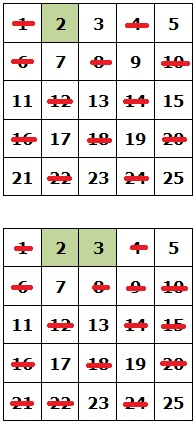
\includegraphics[width=2.5cm]{eratosthenes_02.jpg}
%\caption{Bild1}
%\label{fig:Bild1}
\end{minipage}
\hfill
\begin{minipage}[t]{10cm}
\vspace{0pt}
\begin{itemize}
	\item The sieve starts by crossing $1$ from the list, because $1$ is neither prime nor composite.
	\item $2$ is a prime number, hence it remains on the list. 
	\item All multiples of $2$, i.e. $4,\ 6,\ 8,\ 12,\ldots$, are composite, because they can be divided by $2$. They are crossed from the list. 
	\item The next number that is not crossed is $3$, which is prime. All multiples of $3$ up to limit $N$, that are not already crossed, are removed from the list.
\end{itemize}
\end{minipage}
\end{figure}
\vspace{-0.8cm}
\begin{figure}[htbp]
\begin{minipage}[t]{1cm}
\vspace{0pt}
\centering
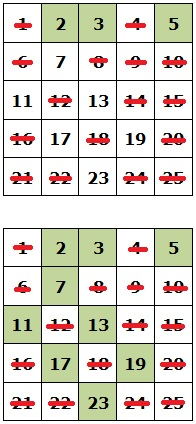
\includegraphics[width=2.5cm]{eratosthenes_03.jpg}
%\caption{Sieve}
%\label{fig:Bild1}
\end{minipage}
\hfill
\begin{minipage}[t]{10cm}
\vspace{0pt}
\begin{itemize}
	\item The next number that is not crossed is $5$, hence $5$ is a prime number. Again, its multiples are removed from the list. 
	\item The next number still on the list is $7$. But $7^2=49$ is larger than $25$. Thus, no multiples of $7$ have to be crossed from the list
			because the lower multiples ($2\cdot 7,\ 3\cdot 7,\ 4\cdot 7$)  are also multiples of $2$ and $3$. Therefore, they are already removed from the list.
	\item The algorithm stops here. All remaining numbers on the list are prime numbers.
\end{itemize}
\end{minipage}
\end{figure}

\noindent The main idea of the method is that every considered number $p$ will be prime. The sieve crosses all multiples of that prime from the list and examines the next number $p$ still on the list. It terminates when $p^2$ is larger than the limit $N$. A slight modification of the sieve of Eratosthenes allows to find the prime factorizations for each integer between $1$ and some bound $N$. The appendix holds a short description of this variation of the sieve. 

%%%%%%%%%%%%%%%%%%%%%%%%%%%%%%%%%%%%%%%%%%%%%%%%%%%%%%%%%%%%%%%%%%%%%%%%
% Sieve of Atkin and Bernstein
%%%%%%%%%%%%%%%%%%%%%%%%%%%%%%%%%%%%%%%%%%%%%%%%%%%%%%%%%%%%%%%%%%%%%%%%

\subsection{Sieve of Atkin and Bernstein}

The sieve of Eratosthenes is not optimal. For instance it needs a large amount of memory. Therefore, in 2004 a new algorithm was introduced by Arthur O.L. Atkin and Daniel J. Bernstein. This algorithm does not make use of the divisibility characterization of primes. It is based on the fact that all prime numbers except 2 and 3 are element of one of the following three sets: 
\begin{itemize}
	\item \textbf{Group 1:} $\left\{n\in\mathbb{N}\ |\ n\equiv 1\ \left(mod\ 4\right)\right\} $
	\item \textbf{Group 2:} $\left\{n\in\mathbb{N}\ |\ n\equiv 1\ \left(mod\ 6\right)\right\} $
	\item \textbf{Group 3:} $\left\{n\in\mathbb{N}\ |\ n\equiv 11\ \left(mod\ 12\right)\right\} $
\end{itemize}
\\
\textbf{Remark 1.} A number $n\in\mathbb{N}$ is called \textbf{congruent to k modulo m}, if $(n-k)$ is divisible by $m$, or equivalently if $n=s\cdot m + k$ for some $s\in\mathbb{Z}$. Then the following notation is used: $n\equiv k\ \left(mod\ m\right)$.
The expression $n\equiv k\ \left(mod\ m\right)$ basically means that both $n$ and $k$ yield the same remainder, if they are divided by $m$. Especially if $k<m$ holds true, then dividing $k$ by $m$ results in the remainder $k$. Since $n$ has the same remainder as $k$ if divided by $m$, this implies that all integers $n$ with $n\equiv k\ \left(mod\ m\right)$ yield remainder $k$ if divided by $m$. \\
\\
\textbf{Example:}
\begin{itemize}
 \item $15\equiv 12\ (mod\ 3)$, because $15-12=3$ is divisible by $3$. Both, $15$ and $12$ yield remainder $0$ if divided by $3$.
 \item $11\equiv 2\ (mod\ 3)$, because $11-2=9$ is divisible by $3$. Both, $11$ and $2$ give remainder $2$ if divided by $2$.
\end{itemize}

% Quelle Remark und Bsp.: 'A readable introduction to real mathematics'
% Evtl. eigene Beispiele ausdenken!!!

%%%%%%%%%%%%%%%%%%%% Theory behind the Algorithm %%%%%%%%%%%%%%%%%%%%%%%

\subsubsection{Theory behind the Algorithm}

The algorithm is based on the following three theorems. Each theorem corresponds to one of the groups above.\\
\\
\noindent \textbf{Theorem 2.1.}
\textit{Let n be a squarefree positive integer with $n\equiv 1\ \ (mod\ 4)$. Then n is prime if and only if the cardinality of the following set is odd:} 
\begin{equation*}
	\left\{\left(x,y\right)\ |\ 4x^2+y^2=n,\ x>0,\ y>0\right\}
\end{equation*}

\noindent \textbf{Remark 2.} A \textbf{squarefree number} is an integer, which is divisible by no other square number than $1$. Equivalently, an integer is squarefree if and only if no prime factor occurs more than once in its prime factorization. \\
\\
The above theorem basically states that a squarefree, positive integer $n$ which is congruent to $1\ (mod\ 4)$ is a prime number if and only if the number of possible solutions $(x,y)$ to the quadratic form $4x^2+y^2=n$ is odd, where $x$ and $y$ are positive integers. Similar results can be found for numbers that are congruent to $1\ (mod\ 6)$ and to $11\ (mod\ 12)$.\\
\\
\noindent \textbf{Theorem 2.2.}
\textit{Let n be a squarefree positive integer with $n\equiv 1\ \ (mod\ 6)$. Then n is prime if and only if the cardinality of the following set is odd:} 
\begin{equation*}
	\left\{\left(x,y\right)\ |\ 3x^2+y^2=n,\ x>0,\ y>0\right\}
\end{equation*}

\noindent \textbf{Theorem 2.3.}
\textit{Let n be a squarefree positive integer with $n\equiv 11\ \ (mod\ 12)$. Then n is prime if and only if the cardinality of the following set is odd:} 
\begin{equation*}
	\left\{\left(x,y\right)\ |\ 3x^2-y^2=n,\ x>y>0\right\}
\end{equation*}

\noindent Proofs for all three theorems can be found in \cite{Atkin03}.

%%%%%%%%%%%%%%%%%%%%%%%%%%%% Representations %%%%%%%%%%%%%%%%%%%%%%%%%%%

\subsubsection{Reformulation of Groups}

It can be shown that all numbers that are either congruent to $1\ \left(mod\ 4\right)$, to $1\ \left(mod\ 6\right)$ or to $11\ \left(mod\ 12\right)$ are also congruent to $r\ \left(mod\ 60\right)$, implying that they can be represented in the form $60k + r$ with varying values for $r$. Therefore, it suffices to consider the following three sets of numbers to find all prime numbers. A derivation of these three sets is provided in the appendix.

\begin{itemize}
	\item \textbf{Group 1:} $\left\{60k + r\ |\ k\in\mathbb{N},\ r\in\left\{1,13,17,29,37,41,49,53\right\}\right\}$
	\item \textbf{Group 2:} $\left\{60k + r\ |\ k\in\mathbb{N},\ r\in\left\{7,19,31,43\right\}\right\}$
	\item \textbf{Group 3:} $\left\{60k + r\ |\ k\in\mathbb{N},\ r\in\left\{11,23,47,59\right\}\right\}$
\end{itemize}

\noindent These representations are more convenient to use in the algorithm. To test an integer $n$ for primality, one simply has to divide it by $60$ and check if the remainder $r$ is in one of the above remainder-sets. Then, the respective theorem can be applied.

%%%%%%%%%%%%%%%%%%%%%%%%%%%% Algorithm %%%%%%%%%%%%%%%%%%%%%%%%%%%%%%%%%

\subsubsection{Algorithm}

\begin{enumerate}
	\item A sieve list is created, containing the entry 'prime' or 'non prime' for each integer from $1$ up to limit $N$. Each number is initially marked as non prime, except for $2$, $3$ and $5$ which are marked as 'prime'.
	\item For each $n\leq N$ the modulo-$60$ remainder of $n$ is calculated. Then, the remainder $r$ is considered.
		\begin{itemize}
			\item \textbf{If} $\boldsymbol{r\in\{1,13,17,29,37,41,49,53\}}$: \\ The $n^{th}$ entry in the sieve list is changed from prime to non prime (or vice versa) for all $\left(x,y\right)$ with $x,y>0$ where $4x^2+y^2=n$.
			\item \textbf{If} $\boldsymbol{r\in\{7,19,31,43\}}$: \\ The $n^{th}$ entry in the sieve list is changed from prime to non prime (or vice versa) for all $\left(x,y\right)$ with $x,y>0$ where $3x^2+y^2=n$.
			\item \textbf{If} $\boldsymbol{r\in\{11,23,47,59\}}$: \\ The $n^{th}$ entry in the sieve list is changed from prime to non prime (or vice versa) for all $\left(x,y\right)$ with $x>y>0$ where $3x^2-y^2=n$.
		\end{itemize}
 \item The algorithm takes the smallest number $p_1$ which was marked as prime in step 2. The entry for all multiples of the square of $p_1$ ($p_1^2,\ 2p_1^2,\ 3p_1^2,\ldots $) is changed to non prime. Then the next larger prime number $p_2$ is considered and multiples of $p_2^2$ are marked as non prime. This step will be repeated until $p_k^2 > N$ for some $k\in\mathbb{N}$.
\end{enumerate}
The last step is important, because the three theorems only apply to squarefree integers. After applying them to the three groups of numbers, there are still non-squarefree integers that could wrongly be marked as prime numbers. 

%%%%%%%%%%%%%%%%%%%%%%%%%%%%% Example %%%%%%%%%%%%%%%%%%%%%%%%%%%%%

\subsubsection{Example}

With the sieve of Atkin and Bernstein, it is very easy to check if any number $n\in\mathbb{N}$ is prime:

\begin{itemize}
	\item \underline{\textbf{n=7:}} Division by $60$ yields the modulo-remainder $r=7$. It is in the remainder-set of the second group of numbers. There is only one possible solution to the quadratic form $3x^2+y^2=n$ where $x$ and $y$ are positive integers: $x=1$ and $y=2$. This is an odd number of solutions, thus $n=7$ is prime.
		\item \underline{\textbf{n=61:}} Division by $60$ yields the modulo-remainder $r=1$. It is in the remainder-set of the first group of numbers. There is only one possible solution to the quadratic form $4x^2+y^2=61$ where $x$ and $y$ are positive integers: $x=3$ and $y=5$. This is an odd number of solutions, thus $n=61$ is prime.
\end{itemize}
				
%%%%%%%%%%%%%%%%%%%%%%%%%%%%%%%%%%%%%%%%%%%%%%%%%%%%%%%%%%%%%%%%%%%%%%%%
% Finding Large Prime Numbers
%%%%%%%%%%%%%%%%%%%%%%%%%%%%%%%%%%%%%%%%%%%%%%%%%%%%%%%%%%%%%%%%%%%%%%%%

\section{Finding Large Prime Numbers}

The described methods have been implemented in R and used to find large prime numbers\footnote{The R-Codes can be found here: \url{https://github.com/kraftjos/NIC_project_Kraft/tree/master/R-Codes} (Last update: 28.02.2016)}. Results of these simulations are shown in this section, and a comparison of the methods is provided.

%%%%%%%%%%%%%%%%%% Simulations %%%%%%%%%%%%%%%%%%%%%%%%%%%%%%%%%%%%%%%%%

\subsection{Simulations}

The implementation of the sieve of Eratosthenes resulted in a simple R-code. It returns a vector of all prime numbers up to limit $N$. At first, a vector $a$ is defined consisting of all numbers that will be checked for primality, i.e. all integers from $2$ up to limit $N$. An empty vector $r$ is generated, which in the end contains all prime numbers found. Then, a while-loop is used, that terminates when $p^2>N$. Inside the loop, the first element of the vector $a$ will be added to the results vector $r$, because the first element of $a$ will always be a prime number. Then it is tested for which elements of the vector $a$ the division by $p$ has remainder $0$. Those elements are multiples of $p$ and will be removed from the vector. Now, the first element of the new vector will be a new prime number. 
The sieve is not implemented exactly as described in \textbf{Section 3.1}, but since R offers the possibility of logical indexing, it is more convenient to implement the method in this way instead of using an additional loop that removes all multiples of $p$ from the list by sequentially adding $p$. \\
\\
The implementation of the sieve of Atkin and Bernstein in R is more complex. At first the vector $to\_test$ is created consisting of numbers of the form $60\cdot k + r$ with $r$ in one of the three remainder-sets described in \textbf{Section 3.2}. All numbers except for $2$, $3$ and $5$ will be marked as non prime in the vector $is\_prime$. The modulo-$60$ remainders for all numbers are calculated and the respective theorem from \textbf{Section 3.2.1} is applied depending on the remainder-set that contains $r$. For each theorem, the respective quadratic form is defined as a function depending on $y$. The corresponding $x$-value is calculated by evaluating the function at all integer values between $1$ and $\sqrt{n}$. Here $n$ is the number checked for primality. The number of $x$-values that are of type integer is counted. If the count is odd, the corresponding value in $is\_prime$ is changed to TRUE. In the end, all non-squarefree numbers that were wrongly marked as prime will be removed from the list.\\
\\
The implementations of the sieve of Eratosthenes and the sieve of Atkin and Bernstein gave the following results:

\begin{table}[!h]
\begin{tabular}{lll}
	\hline
	Test for $N=10^8$	& \textbf{Eratosthenes} & \textbf{Atkin \& Bernstein} \\
	\hline \hline
	\textbf{Primes found} &  5,761,455 & 5,761,455 \\
	\textbf{Largest Prime} & 99,999,989 & 99,999,989 \\
	\textbf{Running Time} & 4.5 min & 6.2 hours \\
	\hline
\end{tabular}\\
\begin{tabular}{ll}
	\hline
	Test for $N=10^9$	& \textbf{Eratosthenes} \\
	\hline \hline
	\textbf{Primes found} &  50,847,534 \\
	\textbf{Largest Prime} & 999,999,937 \\
	\textbf{Running Time} & 1.7 hours \\
	\hline
\end{tabular} 
\caption{Results of Simulations}
\end{table}
\vspace{0cm}
\noindent These results were obtained by using the servers of the ``Research Data Center'' of Humboldt-University in Berlin. Both methods gave the same result for $N=10^8$. The sieve of Atkin and Bernstein needed more than $6$ hours to compute all prime numbers, because the implementation is not very efficient. An efficient implementation of the algorithm is provided by Daniel J. Bernstein on his website\footnote{https://cr.yp.to/primegen.html (Last visit: 28.02.2016)}. 

%%%%%%%%%%%%%%%%%%%%%%%%% Comparison of Methods %%%%%%%%%%%%%%%%%%%%%%%%

\subsection{Comparison of Methods}

The general advantage of sieving is that the arithmetic operations for each number can be small and even bounded. Still, there are slight differences between the sieve of Eratosthenes and the sieve of Atkin and Bernstein concerning computational efficiency.\\
\\
\textbf{Sieve of Eratosthenes:}\\
The algorithm starts with $p$ and adds $p$ sequentially until limit $N$ to remove all multiples. Hence, all arithmetic operations needed are additions. According to \cite{Crandall05}, it can be shown that the number of steps is proportional to 
\begin{equation*}
	\sum_{p\leq N} \frac{N}{p} = N \cdot \ln{\ln{N}} + \mathcal O(N)
\end{equation*}
Therefore, the sieve has a complexity of $\mathcal O(N\cdot \ln{\ln{N}})$.\\
\\
As stated in \cite{Joux09}, the sieve of Eratosthenes has two main limitations. One is the high computational cost which derives from the fact that small prime numbers have many multiples, thus sieving the smaller primes is the costly part. A way to avoid this is for instance to remove all even numbers except $2$. This implies that if $x$ is an odd multiple of $p$, then $x+p$ will be even and thus not considered by the algorithm. The sieve directly examines $x+2p$ and crosses this number from the list, i.e. marks it as non prime. In this way, it is possible to consider up to twice as many numbers as before, needing the same time and memory. Wheel factorization enhances this basic idea, because it allows to skip sieving over all muliples of some lower primes (e.g. $2$, $3$, $5$, ...) that are more costly.\\ 
\\
Another drawback of the sieve of Eratosthenes is the large amount of memory needed, because it needs to store the boolean variable ('prime' or 'non prime') for every number up to the limit. This implies that for instance with $1$ GB memory it is not possible to compute primes higher than $2^{33}$. To overcome this limitation, the segmented sieve of Eratosthenes was presented. For instance, it allows to compute all primes until limit $N=2^{34}$ using $2^{17}$ bits of memory. Here, the considered limit $N$ is already higher than the maximal bound in the usual sieve of Eratosthenes. In general, it is very difficult to create an algorithm based on Eratosthenes' sieve that has improved complexity and doesn't need a large amount of memory. Paul Pritchard was able to propose a modified version of the sieve that requires only $\mathcal O(\frac{N}{\ln{\ln{N}}})$ steps and $N^{1+o(1)}$ bits of memory. For details see \cite{Pritchard81}.\\
\\
\noindent\textbf{Sieve of Atkin and Bernstein:}\\
According to \cite{Joux09} the main limitation is that until today no algorithm based on the sieve of Eratosthenes achieves a small running time and simultaneously uses only a small amount of memory. The algorithm of Atkin and Bernstein solves this problem. An efficiently implemented algorithm based on Atkin and Bernstein outperforms the best algorithm based on Eratosthenes with a running time of $\mathcal O(\frac{N}{\ln{\ln{N}}})$ and using $N^{\frac{1}{2}+o(1)}$ bits of memory, as stated in \cite{Atkin03}. 


%%%%%%%%%%%%%%%%%%%%%%%%%%%%%%%%%%%%%%%%%%%%%%%%%%%%%%%%%%%%%%%%%%%%%%%%
% Final Conclusions
%%%%%%%%%%%%%%%%%%%%%%%%%%%%%%%%%%%%%%%%%%%%%%%%%%%%%%%%%%%%%%%%%%%%%%%%

\section{Conclusion}

Prime numbers are essential for encryption methods. Thus, the interest in prime number theory and prime generating algorithms has grown rapidly in the past years. Besides the sieve of Atkin and Bernstein, many other algorithms have been developed to find prime numbers. Nevertheless, the sieve of Eratosthenes was best concerning computational cost for a very long time, even though it is a very simple method with a straightforward implementation. \\
\\
The sieve of Atkin and Bernstein is not able to outperform the sieve of Eratosthenes when only the running time is of interest. However, it is able to achieve the same bound for computation time and simultaneously optimize the memory needed. At the time when Atkin and Bernstein presented their sieve, no other method was able to do this, which makes it one of the best methods to find large prime numbers so far.\\
\\
Apart from algorithms that generate prime numbers, researchers are interested in methods that find prime factorizations of numbers. As stated in \cite{Crandall05} there are exponential factoring algorithms, i.e. if $n$ is the number that needs to be factored, the running time is bounded by $n^a$ for some fixed, positive number $a$. Only in the $1970$s, subexponential factoring algorithms such as the quadratic sieve factorization method were introduced. Still, those methods are in general much slower than those that generate primes. In particular, it would take an immense amount of time to find the factorization for very large numbers. Therefore, encryption methods based on prime numbers are currently secure. However, the growing need for information security makes further developments of prime generating algorithms essential.   

%%%%%%%%%%%%%%%%%%%%%%%%%%%%%%%%%%%%%%%%%%%%%%%%%%%%%%%%%%%%%%%%%%%%%%%%
% Appendix
%%%%%%%%%%%%%%%%%%%%%%%%%%%%%%%%%%%%%%%%%%%%%%%%%%%%%%%%%%%%%%%%%%%%%%%%

\newpage

\pagenumbering{Roman}
\setcounter{page}{4}

\section{Appendix}

\subsection{Proof of the Fundamental Theorem of Arithmetic}

The follwing proof is based on \cite{Rosenthal14}:\\
\\
\textbf{\textit{Proof.}}\\
\\
1. To prove the existence of a prime factorization, assume that there is at least one integer larger than one such that it can not be represented as a product of primes. Then, there is a smallest number $n$ having this property. Since $n$ is not a prime number (otherwise $n=n$ would be the required prime factorization), there exist integers $k$ and $l$ such that $n=kl$ with $1<k,l<n$. Because $n$ is the smallest number without a prime factorization, both $k$ and $l$ can be written as a product of primes:
\begin{equation*}
k=p_1\cdot\ldots\cdot p_s \hspace{2cm} l=q_1\cdot\ldots\cdot q_t
\end{equation*}
Thus, $n$ can be represented as $n=p_1\cdot\ldots\cdot p_s\cdot q_1\cdot\ldots\cdot q_t$. Hence, a prime factorization for $n$ was found. $\lightning$ \\
\\
2. To prove the uniqueness of the representation (except for the order of the primes), assume that there is at least one natural number $n$ with two different representations:
\begin{equation*}
n=p_1\cdot\ldots\cdot p_k=q_1\cdot\ldots\cdot q_l
\end{equation*}
with $p_1,\ldots ,p_k$ and $q_1,\ldots ,q_l$ being prime numbers. Assume that $n$ is the smallest number with no unique prime factorization. Then $p_i\neq q_j$ for all $i,j$ because if $p_i=q_j$ for some $i,j$ then division of $n$ by $p_i$ would result in a number smaller than $n$ with no unique prime factorization. But it was assumed that $n$ is the smallest number with this property.\\
\\
Since $p_1\neq q_1$, suppose without loss of generality that $p_1<q_1$. Define
\begin{equation*}
\begin{align*}
m&:=n-(p_1\cdot q_2\cdot\ldots\cdot q_l) \\
 &= (p_1\cdot\ldots\cdot p_k)-(p_1\cdot q_2\cdot\ldots\cdot q_l) \\
 &= p_1\cdot\left\{\left(p_2\cdot\ldots\cdot p_k\right)-\left(q_2\cdot\ldots\cdot q_l\right)\right\} \\
\end{align*}
\end{equation*}
Obviously $p_1$ divides $m$, hence $m\neq1$. Because $m<n$, $m$ has a unique factorization into prime numbers. But $m$ can also be written as
\begin{equation*}
\begin{align*}
m&=(q_1\cdot\ldots\cdot q_l)-(p_1\cdot q_2\cdot\ldots\cdot q_l) \\
 &= (q_1-p_1)\cdot (q_2\cdot\ldots\cdot q_l)
\end{align*}
\end{equation*}
%To find the unique prime factorization of m, one needs to find the unique factorization of $(q_1-p_1)$. 
Since $p_1$ is a divisor of $m$, it must appear in the unique factorization. It holds that $p_1\neq q_j$ for all $j$, therefore $p_1$ must occur in the unique factorization of $(q_1-p_1)$. This means:
\begin{equation*}
q_1-p_1=s\cdot p_1, \hspace{1cm} s\in\mathbb{N}
\end{equation*}
It follows that
\begin{equation*}
\begin{align*}
q_1&= p_1+p_1\cdot s \\
   &= p_1\cdot (1+s)
\end{align*}
\end{equation*}
Hence $q_1$ is divisible by $p_1$. But $q_1$ is a prime number. $\lightning$
\qed\\
\\
% Quelle Beweis: 
% Existenz: www.math.hawaii.edu/~lee/courses/fundamental.pdf
% Eindeutigkeit: 'A Readable Introduction to Real Mathematics', 
% von Daniel Rosenthal, David Rosenthal, Peter Rosenthal
% Springer Verlag 2014

\subsection{Complete Factorizations with the Sieve of Eratosthenes}

The sieve of Eratosthenes is useful to find prime factorizations. The following simple example illustrates the algorithm. It computes the prime factorizations for all numbers between $1$ and $9$.\\
\vspace{-0.5cm}
\begin{figure}[!h]
\centering
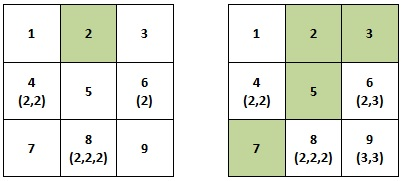
\includegraphics[width=8cm]{factorization_new.jpg}
\end{figure}\\
\vspace{-0.5cm}
\\
\noindent As can be seen in the figure above, the first step of the algorithm starts by marking $2$ as prime number. Instead of crossing all multiples of $2$ from the list, a $2$ is added in parentheses for each multiple of $2$, since every multiple has $2$ as a prime factor. Next, an additional $2$ is written in parentheses under each multiple of $2^2$. In this case, the multiples are $4$ and $8$. These multiples have at least two prime factors that are equal to $2$. The same is repeated with $2^3$. Multiples will receive an additional $2$ in parentheses. Here, the only multiple of $2^3$ is $8$, thus a $2$ is added in parentheses. Since $2^4>9$, the algorithm continues with the next prime number which is $3$. Thus, in the second step, $3$ will be marked as prime number. All multiples of $3$ will receive a $3$ in parentheses, because they have $3$ as prime factor. In this example, these multiples are $6$ and $9$. Next, an additional $3$ is added in parentheses to $9$, because $9$ is a multiple of $3^2$. As $3^3>9$ and since the next prime number is $5$ with $5^2>9$, the algorithm stops here.\\
\\
\noindent In general, the algorithm computes prime factorizations for all numbers from $1$ up to limit $N$. It always considers primes $p$ and adds $p$ in parentheses for multiples of $p^k$ for $k\in\mathbb{N}$ until $p^k>N$ for some $k$. Then it continues with the next larger prime number $p$. The algorithm stops if $p^2>N$ for some prime number $p$.

\subsection{Reformulation of Groups in the Sieve of Atkin and Bernstein}

Consider the first set of numbers, denoted by $M_1$, that is considered in the sieve of Atkin and Bernstein:
\begin{equation*}
\begin{align*}
M_1&\stackrel{\operatorname{def}}{=}\left\{n\in\mathbb{N}\ |\ n\equiv 1\ \left(mod\ 4\right) \right\} \\
&=\left\{n\in\mathbb{N}\ |\ n=4k+1,\ k\in\mathbb{N} \right\} \\
&=\left\{1,5,9,13,17,21,25,29,33,37,41,45,49,53,57,61,65,69,\ldots \right\}
\end{align*}
\end{equation*}
It contains every 4th number of the natural numbers starting with $1$. The aim is to write this set in the form
\begin{equation*}
\begin{align*}
M_1^&\stackrel{!}{=}\left\{ n\in\mathbb{N}\ |\ n\equiv r\ \left(mod\ 60\right),\ r\in R \right\} \\
&=\left\{ n\in\mathbb{N}\ |\ n=60k+r,\ k\in\mathbb{N},\ r\in R \right\}
\end{align*}
\end{equation*}
for some suitable set $R\subseteq\mathbb{N}$. 
Let $m\in M_1$ with $m<60$. Then division of $m$ by $60$ yields remainder $r=m$. This implies that $m=60\cdot 0 + m$ or $m\equiv m\ \left(mod\ 60\right)$. Therefore, for $m<60$ the set $R^*\subseteq R$ can be defined as:
\begin{equation*}
R^*\stackrel{\operatorname{def}}{=}\left\{1,5,9,13,17,21,25,29,33,37,41,45,49,53,57\right\} 
\end{equation*}
Now, consider all numbers $m\in M_1$ with $60\leq m<2\cdot 60$. The first number is $61=60\cdot 1 + 1$. Thus, it is already of the form $60k+r$ with $r=1$, hence $r\in R^*$. Further, one can see that $65=60\cdot 1 + 5$, $69=60\cdot 1 + 9$, and so on. Obviously, it holds $m=60\cdot 1 + r$ with $r\in R^*$ for all $m\in M_1$ with $60\leq m<2\cdot 60$. Similarly, for all $m\in M_1$ with $2\cdot 60 \leq m<3\cdot 60$ it holds $m=60\cdot 2 + r$ with $r\in R^*$. For instance, $121=60\cdot 2 + 1$, $125=60\cdot 2 + 5$, and so on. In general, for all numbers $m_z\in M_1$ with $z\cdot 60\leq m_z < \left(z+1\right)\cdot 60$ and $z\in\mathbb{N}$ it holds: $m_z=60\cdot z + r$ with $r\in R^*$. Therefore, $R^*=R$ and one can write 
%Note that the following rule holds true: $r+k\cdot m\equiv r\ \left(mod\ m\right)$ for $k\in\mathbb{Z}$.
\begin{equation*}
\begin{align*}
	M_1&=\big\{n\in\mathbb{N}\ |\ n\equiv r\ \left(mod\ 60\right), \\
	&\qquad r\in\left\{1,5,9,13,17,21,25,29,33,37,41,45,49,53,57 \right\} \big\}
	\end{align*}
\end{equation*}
Analogously, one can see that for the second group of numbers from the sieve of Atkin and Bernstein it holds
\begin{equation*}
\begin{align*}
M_2	&=\left\{ n\in\mathbb{N}\ |\ n\equiv 1\ \left(mod\ 6\right)\right\} \\
		&=\left\{ n\in\mathbb{N}\ |\ n=6k+1,\ k\in\mathbb{N}\right\} \\
		&=\left\{1,7,13,19,25,31,37,43,49,55,61,\ldots \right\}
\end{align*}
\end{equation*}
The set corresponds to every 6th natural number starting with $1$. Similarly to $M_1$, it can be written as
\begin{equation*}
M_2=\left\{n\in\mathbb{N}\ |\ n=60k+r, k\in\mathbb{N}, r\in\left\{1,7,13,19,25,31,37,43,49,55\right\} \right\}
\end{equation*}
In the same way, all numbers $n$ from the third group of numbers with $n$ congruent to $11\ \left(mod\ 12\right)$ can be represented as 
\begin{equation*}
M_3=\left\{n\in\mathbb{N}\ |\ n=60k+r, k\in\mathbb{N}, r\in\left\{11,23,35,47,59\right\} \right\}
\end{equation*}
So far, the remainder-sets for $M_1$, $M_2$ and $M_3$ are the following:
\begin{itemize}
	\item $R_1=\left\{1,5,9,13,17,21,25,29,33,37,41,45,49,53,57 \right\}$
	\item $R_2=\left\{1,7,13,19,25,31,37,43,49,55\right\} \right\}$
	\item $R_3=\left\{11,23,35,47,59\right\} \right\}$
\end{itemize}
The sets $R_1$ and $R_2$ contain overlaps. A remainder can be removed from $R_2$ if it is already contained in $R_1$, because it is not efficient to check a number twice for primality. Hence, the second set reduces to $R_2=\left\{7,19,31,43,55\right\}$.\\
\\
\noindent A final modification can be made in the following way: If there exists an integer $g$ such that $g$ divides $m$ and $r$. Then $g$ also divides $n=m\cdot k\ +\ r$ with $k\in\mathbb{N}_{0}$. This implies that $n$ is not a prime number. In this case $m=60$ has divisors 2, 3 and 5.
In $R_1$ remainders 9, 21, 33, 45, 57 have divisor 3 and remainders 5, 25 and 45 have divisor 5. Thus, they can be removed. Remainder 55 from $R_2$ and remainder 35 from $R_3$ have divisor 5 and can be deleted. This modification yields the final sets that are considered in the sieve of Atkin and Bernstein:
\begin{itemize}
	\item $M_1=\left\{n\in\mathbb{N}\ |\ n=60k+r,\ k\in\mathbb{N},\ r\in\left\{1,13,17,29,37,41,49,53 \right\} \right\}$
	\item $M_2=\left\{n\in\mathbb{N}\ |\ n=60k+r,\ k\in\mathbb{N}, r\in\left\{7,19,31,43\right\} \right\}$
	\item $M_3=\left\{n\in\mathbb{N}\ |\ n=60k+r,\ k\in\mathbb{N}, r\in\left\{11,23,47,59\right\} \right\}$
\end{itemize}     

%%%%%%%%%%%%%%%%%%%%%%%%%%%%%%%%%%%%%%%%%%%%%%%%%%%%%%%%%%%%%%%%%%%
% Bibliographie
%%%%%%%%%%%%%%%%%%%%%%%%%%%%%%%%%%%%%%%%%%%%%%%%%%%%%%%%%%%%%%%%%%%

\newpage

\begin{thebibliography}{9}

\bibitem{Rosenthal14}
	\textbf{Daniel Rosenthal, David Rosenthal, P. Rosenthal:}
	\emph{``A Readable Introduction to Real Mathematics''},
	Springer,
	2014.

\bibitem{Atkin03}
	\textbf{A.O.L. Atkin, D.J. Bernstein:}
	\emph{``Prime Sieves Using Binary Quadratic Forms''}, 
	Mathematics of Computation, Volume 73, Number 246, p. 1023-1030,
	2004.
	
\bibitem{Crandall05}
	\textbf{R. Crandall, C. Pomerance:}
	\emph{``Prime Numbers. A Computational Perspective''},
	Springer,
	2005.
	
\bibitem{Joux09}
	\textbf{A. Joux:}
	\emph{``Algorithmic Cryptanalysis''},
	Chapman Hall/CRC,
	2009.
	
\bibitem{Pritchard81}
	\textbf{P. Pritchard:}
	\emph{``A sublinear additive sieve for finding prime numbers''},
	Communications of the ACM, Volume 24, p. 18-23,
	1981.
	
\end{thebibliography}

\newpage 

\listoftables

\end{document}